\documentclass{article}
\usepackage[utf8]{inputenc}
\usepackage[a4paper, total={7in, 10in}]{geometry}
\usepackage{xcolor,listings}
\usepackage{graphicx}


\lstset{
  language=Python,
  backgroundcolor = \color{lightgray},
  showspaces=false,
  numbers=left,
  numberstyle=\tiny,
  commentstyle=\color{darkgray},
  keywordstyle=\color{purple}\ttfamily,
  basicstyle=\ttfamily,
  columns=fullflexible,
  frame=single,
  breaklines=true,
  postbreak=\mbox{\textcolor{black}{$\hookrightarrow$}\space}
}


\title{ \textbf{ Graphics in the Nintendo Entertainment System - NES } }
\author{ Nicolas Novalic }

\begin{document}

\begin{center}
	{\Huge NES Graphics}
\end{center}

\section*{CHR files}

A NES ROM can be split into two files, whose extensions are .PRG and .CHR. Usually the PRG file is the content of the PRG ROM and the CHR file is the content of the CHR ROM, both inside the cartridge. The PRG chip connects to the NES motherboard's CPU and contains the compiled code programmed for the the game, while the CHR chip goes to the PPU (Picture Processing Unit) and contains data for the graphics. The PCBs of the cartridges vary a lot in every game, so the aforementioned is not the rule. But to keep things simple and concise let's imagine that this is always the case.

\begin{figure}[h]
\centering
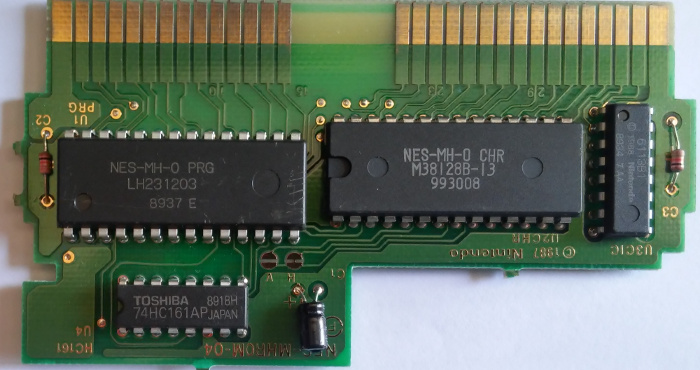
\includegraphics[width=0.8\textwidth]{pcb}
\caption{PCB of a NES cartridge where we can see the CHR and PRG ROMS.}
\end{figure}


The sprites on the NES are 8x8 pixel \textit{tiles}, and actually, the CHR contains the data for each of the tiles that are used on a particular game (and sometimes some that is not used) in a structured way. You can picture the contents of a CHR file as a matrix where the entries are 8x8 pixel tiles. Each tile only has 4 different colors, and usually many tiles are puzzled together to draw a complex shape in the screen.
\vskip 0.2in

The NES was released in 1983, technology back then was very limited compared to what we have nowadays. So it's not hard to realize that the size of a game was HUGE issue. The graphics had to be stored in an optimal way so data occupies the less space in memory as possible. The NES developers worked with hardware limitations in such a way that, for example, the size of the Super Mario Bros.nes file is 41KB. Imagine if we mapped all the stages of this game to computer images. If I take a screen-shot of my current screen on my computer, the file is about 20 times bigger than the size of the whole Super Mario Bros.nes file. 

\vskip 0.2in

Why does this happen? It's reasonable that a screen-shot of my computer is much bigger than the whole game. My screen is displaying millions of colors, when the NES outputs only 64 colors (which there's 56 that are unique). Also, the NES based its screen output on the repetition of a definite amount of tiles, taking care that each of these tiles are stored only once in the game's data. Also, there's an important technique used to store all the graphic data that also reduced notoriously the amount of memory needed. This document's main goal is to describe this technique, which is basically indexed color on sub-palettes based on the 64 color NES palette. Let's imagine this situation: As $2^6 = 64$, to represent one of each of these 64 colors we would need 6 bits. So to represent a tile, we would need $6 \times ( 8 \times 8 ) = 384$ bits. This is a lot of information and a waste of space, since we know that in the NES a tile can't have more than 4 different colors. To optimize this, every pixel is represented in the CHR chip with only 2 bits, so we only need 128 bits for each tile (thats $\frac{1}{3}$ of what we needed before!). This means that if we assign a color to each of these $2^2 = 4$ combinations, all the pixels in a CHR would have only 4 different colors. The way the NES has to decode the original colors for each tile is to assign a 'sub-palette' to each tile. A sub-palette has only 4 colors, taken from the 64 color NES palette, and these sub-palette / tile mapping are defined in the PRG chip.
\vskip 0.2in

\newpage

\begin{figure}[h]
\centering
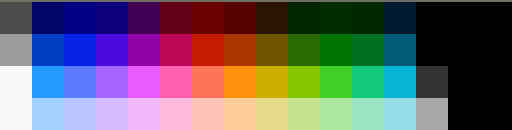
\includegraphics[scale=0.5]{nespalette}
\caption{NES palette.}
\end{figure}


\textbf{A quick example:}
Imagine that the first 8 pixels of a tile are encoded with 01 00 00 00 11 11 11 10. Then suppose that the sub-palette mapped to this particular tile is 000110 110101 010101 000001, which represents a color from the 64 color palette. Then, with this mapping, the real colors of the first 8 pixels of the tile are: 110101 000110 000110 000110 000001 000001 000001 010101. This is, the first pixel is the color in the position 1 of the sub-palette: as positions are numbered from 0 to 3, thats 110101. The second, third and fourth pixels are the color in the position 0 of the sub-palette (000110). Fifth, sixth and seventh are the color in the position 3 of the sub-palette (000001). And the eight pixel is the color in the position 2 in the sub-palette (110101).
\vskip 0.2in
So basically each pixel is represented by an index for its corresponding palette. Knowing the corresponding palette would allow you to know the real color of the pixel, but for this you would need access to the game's code (not compiled).

\begin{figure}[h]
\centering
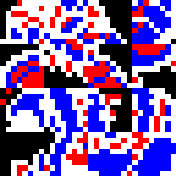
\includegraphics[scale=0.5]{graphics}
\caption{This example gives you an idea of how we can represent data obtained from a CHR file. Here we can see 16 tiles where color 00 is black, 01 is red, 10 blue and 11 is white.}
\end{figure}

\begin{figure}[h]
\centering
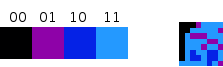
\includegraphics[scale=0.5]{mapping}
\caption{This shows in a graphical way a sub-palette mapped to the first tile from Figure 3. To the left we can see the palette and to the right the tile as we would see it on screen.}
\end{figure}

\vskip 0.2in

Now let's examine the contents of a CHR file. If you open one of these files you will find a large set of hexadecimal numbers. You can see these numbers are structured in a certain way. Remember that we earlier pictured the contents of a CHR file as matrix of tiles? The data inside these files is actually organized as huge matrix of 8 columns and $n$ rows. The amount of rows varies and depends of the amount of graphics the game has. Each entry in this matrix consists of four hexadecimal digits.

A portion of the contents of a CHR file could be:

\begin{lstlisting}
  0000 0000 0000 0000 0000 0000 0000 0000
  0000 0000 0000 0000 0000 0000 0000 0000
  070f 3f7f ffff ff7f 0007 0f37 7f7f 6f1f
  3f3f 1e1c 1c30 70fc 1e1c 0d0b 030f 2f73
  60f0 f8f8 feff ffff 0060 f0e0 f8e0 8000
  c033 73f7 f7f7 3241 3fcc be49 4949 ffbe
  0000 0000 f0e0 d0f0 0000 0000 0000 0000
  e040 8080 80c0 6070 0080 0000 0000 80a0
\end{lstlisting}

\vskip 0.2in

This is actually a small portion of the CHR file of the game Panic Restaurant - this game's CHR file is a 8192x8 matrix. In general, each row of these matrices represents one 8x8 pixel tile, encoded in a certain way. If we decode these matrices we are actually obtaining the all the uncolored tiles of a video-game. To understand the decoding process, we'll go through an example. Let's decode the values for each pixel of the tile from the row six of the excerpt of Panic Restaurant's matrix: \textbf{c033 73f7 f7f7 3241 3fcc be49 4949 ffbe}.
\vskip 0.2in

First, let's split the original row in two parts and place them like this:

\begin{lstlisting}
c033 73f7 f7f7 3241
3fcc be49 4949 ffbe
\end{lstlisting}
\vskip 0.2in

Then, let's obtain the binary representation for each entry of the row:

\vskip 0.2in
\begin{lstlisting}
  0xC033 = 1100000000110011b
  0x73F7 = 0111001111110111b
  0xF7F7 = 1111011111110111b
  0x3241 = 0011001001000001b
  0x3FCC = 0011111111001100b
  0xBE49 = 1011111001001001b
  0x4949 = 0100100101001001b
  0xFFBE = 1111111110111110b
\end{lstlisting}
\vskip 0.2in

And replace the split row with its binary representation:

\begin{lstlisting}
1100 0000 0011 0011 0111 0011 1111 0111 1111 0111 1111 0111 0011 0010 0100 0001
0011 1111 1100 1100 1011 1110 0100 1001 0100 1001 0100 1001 1111 1111 1011 1110
\end{lstlisting}
\vskip 0.2in

Notice that here we had added a white-space between each hex digits binary representation for a better appreciation. Also we can see that we have 128 bits of data, which is the amount of bits we calculated before that would be needed for a tile.

\vskip 0.2in

So in each part of the split row we have 64 bits. As each tile is 8x8 = 64 pixels, this suggests there is a relation between each part of the split row. The relation is very simple and it's based on the position of each bit. From now on, let's think about the two parts of the split row as line one and line two.
\vskip 0.2in

Imagine each of these lines as two vectors $\phi_1$ and $\phi_2$. Each bit for each line (excluding the white-spaces we added on purpose) is an element on its corresponding vector. In fact lets force that the elements of the vectors appear in the same order as they are on the lines. If any doubt: the value of the element in the position $k$ in the vector is the bit in the $k$ position of its corresponding line (again, excluding white-spaces). Also let's define an access operation/function:

$$\phi_i[j], (i \in \{ 1, 2\}; j \in \{ 1,\dots,64\})$$ 
\vskip 0.2in

that retrieves the decimal number that represents the value of the entry at the $j$ position in the vector $\phi_i$.
\vskip 0.2in

Now, let's define a new vector $\psi$ of length 64, where:

$$ \psi[j] = (\phi_1[j] \times 1) + (\phi_2[j] \times 2) $$
\vskip 0.2in

We have applied a decoding function taking corresponding elements from $\phi_1$ and $\phi_2$ and built a new vector that actually is the representation of a tile. Then if we decompose this vector into an 8x8 matrix we can see the 'shape' of the tile. The function applied to the two vectors is very simple, for each of the 64 possible positions, take the corresponding value from the first vector and add two times the value of the corresponding position in the second vector. The result is the position of the color of the pixel on the corresponding sub-palette. There's two minor things I would like to mention here. First is that $\psi$ is a vector that contains decimal numbers. As we defined the access operation as (some sort of) a function that retrieves a decimal value, the $+$ and $\times$ operations that appear in the decoding function are the base-10 addition and multiplication operators. This is just to make things look nicer. Second thing is that all the possible resulting values of applying this function are $0,1,2,3$, so $\psi[j] \in \{ 0, 1, 2, 3\}$, $j \in \{ 1,\dots,64\}$. 
\vskip 0.2in

For example, the 4th digit of $\phi_1$ is 0, and the 4th digit of $\phi_2$ is 1, so the result is: 

$$(\phi_1[3] \times 1) + (\phi_2[3] \times 2)  = (0 \times 1) + (1 \times 2) = 2$$
\vskip 0.2in

This means the 4th pixel's color is the one in the position $2_{10}$ (or $10_2$) of the tile's corresponding palette. 

\vskip 0.5in

We could calculate the codes for each pixel of the tile by hand pretty easy, but it would be a waste of time. Let's do some \textbf{Python} code to see some quick results:

\begin{lstlisting}
line = 'c033 73f7 f7f7 3241 3fcc be49 4949 ffbe'.replace(' ', '')

result = \
[ x + 2*y for x, y in \
        zip(\
            [int(x) for x in list(bin(int(line[:16], 16))[2:].zfill(64))],\
            [int(x) for x in list(bin(int(line[16:], 16))[2:].zfill(64))]\
        )\
]
\end{lstlisting}

There's a much simpler, explained equivalent version of this code at the end of the document.
\vskip 0.2in

This code outputs the following: \\

[1, 1, 2, 2, 2, 2, 2, 2, 2, 2, 1, 1, 2, 2, 1, 1, 2, 1, 3, 3, 2, 2, 3, 1, 1, 3, 1, 1, 2, 1, 1, 3, 1, 3, 1, 1, 2, 1, 1, 3, 1, 3, 1, 1, 2, 1, 1, 3, 2, 2, 3, 3, 2, 2, 3, 2, 2, 1, 2, 2, 2, 2, 2, 1]
\vskip 0.2in

Which is a position on the sub-palette for each of the 64 pixels of the tile. Let's organize this in an 8x8 matrix:

\begin{lstlisting}
matrix = \
[ result[index:index + 8] for index in range(0, len(result), 8) ]

print(*matrix, sep='\n')
\end{lstlisting}

That code outputs:
\parbox{.45\linewidth}{
\begin{center}
  [1, 1, 2, 2, 2, 2, 2, 2] \\[0pt]
  [2, 2, 1, 1, 2, 2, 1, 1] \\[0pt]
  [2, 1, 3, 3, 2, 2, 3, 1] \\[0pt]
  [1, 3, 1, 1, 2, 1, 1, 3] \\[0pt]
  [1, 3, 1, 1, 2, 1, 1, 3] \\[0pt]
  [1, 3, 1, 1, 2, 1, 1, 3] \\[0pt]
  [2, 2, 3, 3, 2, 2, 3, 2] \\[0pt]
  [2, 1, 2, 2, 2, 2, 2, 1] \\[0pt]
\end{center}
}
\vskip 0.2in

It would be really easy to get the binary representation of each entry if we need to:

\begin{lstlisting}
print(*[ [ bin(entry)[2:].zfill(2) for entry in result ][index:index + 8] \
          for index in range(0, len(result), 8) ], \
      sep='\n'\
    )
\end{lstlisting}

The output is:
\parbox{.45\linewidth}{
\begin{center}
  ['01', '01', '10', '10', '10', '10', '10', '10'] \\[0pt]
  ['10', '10', '01', '01', '10', '10', '01', '01'] \\[0pt]
  ['10', '01', '11', '11', '10', '10', '11', '01'] \\[0pt]
  ['01', '11', '01', '01', '10', '01', '01', '11'] \\[0pt]
  ['01', '11', '01', '01', '10', '01', '01', '11'] \\[0pt]
  ['01', '11', '01', '01', '10', '01', '01', '11'] \\[0pt]
  ['10', '10', '11', '11', '10', '10', '11', '10'] \\[0pt]
  ['10', '01', '10', '10', '10', '10', '10', '01'] \\[0pt]
\end{center}
}

\vskip 0.2in

Note that in this example there's no pixel with the color of position 0 of the sub-palette.

\vskip 0.2in

Let's calculate the colors for each row/tile on the portion of the CHR file originally listed:
\begin{lstlisting}
tiles = ['0000 0000 0000 0000 0000 0000 0000 0000', \
          '0000 0000 0000 0000 0000 0000 0000 0000', \
          '070f 3f7f ffff ff7f 0007 0f37 7f7f 6f1f', \
          '3f3f 1e1c 1c30 70fc 1e1c 0d0b 030f 2f73', \
          '60f0 f8f8 feff ffff 0060 f0e0 f8e0 8000', \
          'c033 73f7 f7f7 3241 3fcc be49 4949 ffbe', \
          '0000 0000 f0e0 d0f0 0000 0000 0000 0000', \
          'e040 8080 80c0 6070 0080 0000 0000 80a0' 
        ]

for tile in tiles:
  line = tile.replace(' ', '')
  result = \
    [ x + 2*y for x, y in \
        zip(\
          [int(x) for x in list(bin(int(line[:16], 16))[2:].zfill(64))], \
          [int(x) for x in list(bin(int(line[16:], 16))[2:].zfill(64))]\
        )\
    ]
  matrix = \
    [ result[index:index + 8] for index in range(0, len(result), 8) ]
  print(*matrix, sep='\n')
  print('\n')
\end{lstlisting}

\parbox{.20\linewidth}{
\begin{center}
	\textbf{tile 1:} \\[2pt]
  [0, 0, 0, 0, 0, 0, 0, 0] \\[0pt]
  [0, 0, 0, 0, 0, 0, 0, 0] \\[0pt]
  [0, 0, 0, 0, 0, 0, 0, 0] \\[0pt]
  [0, 0, 0, 0, 0, 0, 0, 0] \\[0pt]
  [0, 0, 0, 0, 0, 0, 0, 0] \\[0pt]
  [0, 0, 0, 0, 0, 0, 0, 0] \\[0pt]
  [0, 0, 0, 0, 0, 0, 0, 0] \\[0pt]
  [0, 0, 0, 0, 0, 0, 0, 0] \\[0pt]
\end{center}
}
\parbox{.20\linewidth}{
\begin{center}
	\textbf{tile 2:} \\[2pt]
  [0, 0, 0, 0, 0, 0, 0, 0] \\[0pt]
  [0, 0, 0, 0, 0, 0, 0, 0] \\[0pt]
  [0, 0, 0, 0, 0, 0, 0, 0] \\[0pt]
  [0, 0, 0, 0, 0, 0, 0, 0] \\[0pt]
  [0, 0, 0, 0, 0, 0, 0, 0] \\[0pt]
  [0, 0, 0, 0, 0, 0, 0, 0] \\[0pt]
  [0, 0, 0, 0, 0, 0, 0, 0] \\[0pt]
  [0, 0, 0, 0, 0, 0, 0, 0] \\[0pt]
\end{center}
}
\parbox{.20\linewidth}{
\begin{center}
	\textbf{tile 3:} \\[2pt]
  [0, 0, 0, 0, 0, 1, 1, 1] \\[0pt]
  [0, 0, 0, 0, 1, 3, 3, 3] \\[0pt]
  [0, 0, 1, 1, 3, 3, 3, 3] \\[0pt]
  [0, 1, 3, 3, 1, 3, 3, 3] \\[0pt]
  [1, 3, 3, 3, 3, 3, 3, 3] \\[0pt]
  [1, 3, 3, 3, 3, 3, 3, 3] \\[0pt]
  [1, 3, 3, 1, 3, 3, 3, 3] \\[0pt]
  [0, 1, 1, 3, 3, 3, 3, 3] \\[0pt]
\end{center}
}
\parbox{.20\linewidth}{
\begin{center}
	\textbf{tile 4:} \\[2pt]
  [0, 0, 1, 3, 3, 3, 3, 1] \\[0pt]
  [0, 0, 1, 3, 3, 3, 1, 1] \\[0pt]
  [0, 0, 0, 1, 3, 3, 1, 2] \\[0pt]
  [0, 0, 0, 1, 3, 1, 2, 2] \\[0pt]
  [0, 0, 0, 1, 1, 1, 2, 2] \\[0pt]
  [0, 0, 1, 1, 2, 2, 2, 2] \\[0pt]
  [0, 1, 3, 1, 2, 2, 2, 2] \\[0pt]
  [1, 3, 3, 3, 1, 1, 2, 2] \\[0pt]
\end{center}
}
\parbox{.20\linewidth}{
\begin{center}
	\textbf{tile 5:} \\[2pt]
  [0, 1, 1, 0, 0, 0, 0, 0] \\[0pt]
  [1, 3, 3, 1, 0, 0, 0, 0] \\[0pt]
  [3, 3, 3, 3, 1, 0, 0, 0] \\[0pt]
  [3, 3, 3, 1, 1, 0, 0, 0] \\[0pt]
  [3, 3, 3, 3, 3, 1, 1, 0] \\[0pt]
  [3, 3, 3, 1, 1, 1, 1, 1] \\[0pt]
  [3, 1, 1, 1, 1, 1, 1, 1] \\[0pt]
  [1, 1, 1, 1, 1, 1, 1, 1] \\[0pt]
\end{center}
}


\parbox{.20\linewidth}{
\begin{center}
	\textbf{tile 6:} \\[2pt]
  [1, 1, 2, 2, 2, 2, 2, 2] \\[0pt]
  [2, 2, 1, 1, 2, 2, 1, 1] \\[0pt]
  [2, 1, 3, 3, 2, 2, 3, 1] \\[0pt]
  [1, 3, 1, 1, 2, 1, 1, 3] \\[0pt]
  [1, 3, 1, 1, 2, 1, 1, 3] \\[0pt]
  [1, 3, 1, 1, 2, 1, 1, 3] \\[0pt]
  [2, 2, 3, 3, 2, 2, 3, 2] \\[0pt]
  [2, 1, 2, 2, 2, 2, 2, 1] \\[0pt]
\end{center}
}
\parbox{.20\linewidth}{
\begin{center}
	\textbf{tile 7:} \\[2pt]
  [0, 0, 0, 0, 0, 0, 0, 0] \\[0pt]
  [0, 0, 0, 0, 0, 0, 0, 0] \\[0pt]
  [0, 0, 0, 0, 0, 0, 0, 0] \\[0pt]
  [0, 0, 0, 0, 0, 0, 0, 0] \\[0pt]
  [1, 1, 1, 1, 0, 0, 0, 0] \\[0pt]
  [1, 1, 1, 0, 0, 0, 0, 0] \\[0pt]
  [1, 1, 0, 1, 0, 0, 0, 0] \\[0pt]
  [1, 1, 1, 1, 0, 0, 0, 0] \\[0pt]
\end{center}
}
\parbox{.20\linewidth}{
\begin{center}
	\textbf{tile 8:} \\[2pt]
  [1, 1, 1, 0, 0, 0, 0, 0] \\[0pt]
  [2, 1, 0, 0, 0, 0, 0, 0] \\[0pt]
  [1, 0, 0, 0, 0, 0, 0, 0] \\[0pt]
  [1, 0, 0, 0, 0, 0, 0, 0] \\[0pt]
  [1, 0, 0, 0, 0, 0, 0, 0] \\[0pt]
  [1, 1, 0, 0, 0, 0, 0, 0] \\[0pt]
  [2, 1, 1, 0, 0, 0, 0, 0] \\[0pt]
  [2, 1, 3, 1, 0, 0, 0, 0] \\[0pt]
\end{center}
}

\vskip 0.2in

To conclude, by understanding this we know how the graphic data is stored inside the CHR ROM of the NES cartridges and also how the NES works with these graphics. With some work, we could be able to convert our own graphics to NES format. Also, we can read the contents of a CHR file and calculate the position on the sub-palette of each pixel. Note that most of the tiles are placed next to other tiles to create compound, bigger tiles... So if we assign a random color to each different number on a decoded CHR file (4 different numbers = 4 different colors) still many of these tiles would draw reasonable shapes even without their original colors. A nice experiment would be to read the contents of a whole CHR file and process the data. Then we can find tiles that go together and re-build some graphics as characters, items, etc.

\newpage

{\Huge Addendum}

\section*{Resources}

Some useful tools to check out what I wrote in this document.

\subsubsection*{Sublime Text Editor}
This is a nice cross-platform text editor that can open CHR files and display its contents. I've tried other editors such as Atom and Xed and it didn't work well.

\subsubsection*{FamiRom}

This is a nice tool that lets you load a NES ROM file and splits it into PRG and CHR files. The software is for Windows, but you can use it on Linux without problems if you install the package \textbf{mono-complete}. Then just run \textbf{mono famiRom.exe} in the linux console.

\subsubsection*{Python}

A very powerful object oriented programming language.

\section*{Python code for dummies!}

\begin{lstlisting}
# Create two strings with each line of hexadecimal values and removing whitespaces
l1 = 'c033 73f7 f7f7 3241'.replace(' ', '')
l2 = '3fcc be49 4949 ffbe'.replace(' ', '')

# Define a function that given a string representation of a hexadecimal number
# returns a binary string of that number, removing the first two characters that
# are '0b' for binary. Fills with zeros to complete 4 digits.
def to_bin(hexa_num):
  to_int = int(hexa_num, 16)
  return bin(to_int)[2:].zfill(4)

# The function to calculate the color
def calculate(num1, num2):
  return num1 + (2 * num2)
  
# Creating a string of binary digits
# for each line of hexadecimal numbers
bin_string1 = ''
bin_string2 = ''

for index in range(0, 16):
  bin_string1 += (to_bin(l1[index]))
  bin_string2 += (to_bin(l2[index]))

# Turns the strings to lists, then for each entry of the list, converts to 
# integer and apply the function to calculate the resulting color.
list1 = list(bin_string1)
list2 = list(bin_string2)
res = list()

for index in range(0,64):
  num1 = int(list1[index])
  num2 = int(list2[index])
  res.append(calculate(num1, num2))
\end{lstlisting}

\end{document}
